\documentclass{standalone}

\usepackage{tikz}
\usetikzlibrary{automata, positioning}

\begin{document}
    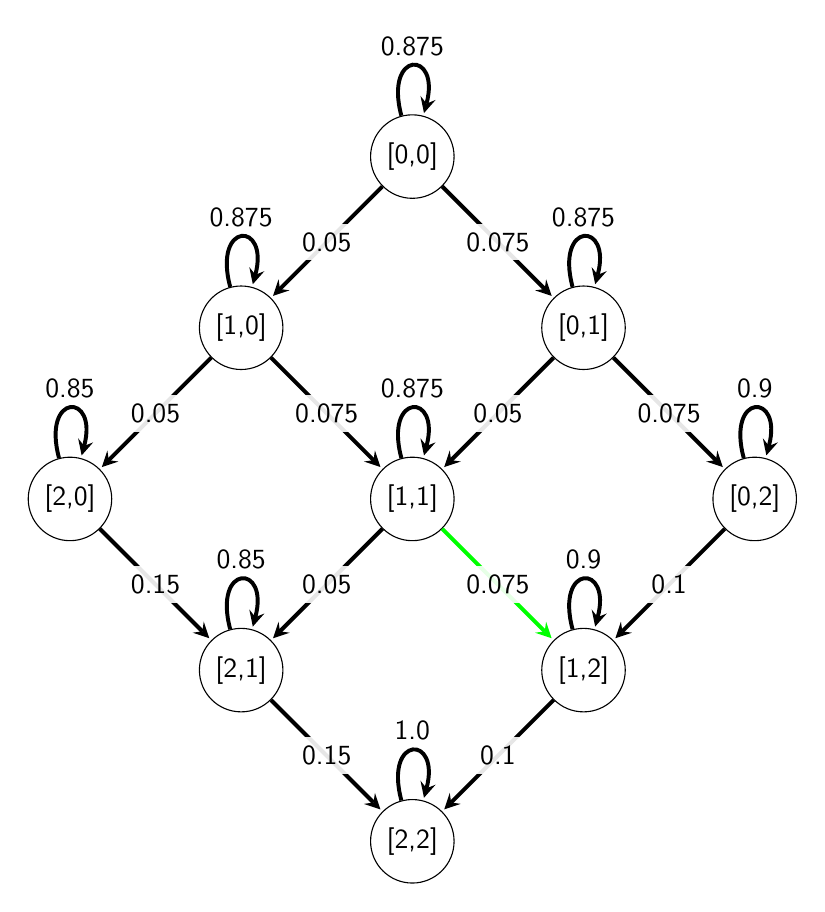
\begin{tikzpicture}[font=\sffamily]

    % Add the states
    \node[state]                          (init)   {[0,0]};
    \node[state, below  left=2cm of init] (a1)     {[1,0]};
    \node[state, below right=2cm of init] (b1)     {[0,1]};
    \node[state, below  left=2cm of b1]   (a1b1)   {[1,1]};
    \node[state, below  left=2cm of a1]   (a2)     {[2,0]};
    \node[state, below right=2cm of b1]   (b2)     {[0,2]};
    \node[state, below right=2cm of a1b1] (a1b2)   {[1,2]};
    \node[state, below  left=2cm of a1b1] (a2b1)   {[2,1]};
    \node[state, below  left=2cm of a1b2] (a2b2)   {[2,2]};

    % Connect the states with arrows
    \draw[every loop,
          line width=.5mm,
          >=stealth,
          draw=black,
          fill=black]
        (init)   edge node[midway, fill=white, fill opacity = 0.9, text opacity=1] {0.05} (a1)
        (init)   edge node[midway, fill=white, fill opacity = 0.9, text opacity=1] {0.075} (b1)
        (a1)     edge node[midway, fill=white, fill opacity = 0.9, text opacity=1] {0.05} (a2)
        (a1)     edge node[midway, fill=white, fill opacity = 0.9, text opacity=1] {0.075} (a1b1)
        (b1)     edge node[midway, fill=white, fill opacity = 0.9, text opacity=1] {0.075} (b2)
        (b1)     edge node[midway, fill=white, fill opacity = 0.9, text opacity=1] {0.05} (a1b1)
        (a1b1)   edge[draw=green] node[midway, fill=white, fill opacity = 0.9, text opacity=1] {0.075} (a1b2)
        (a1b1)   edge node[midway, fill=white, fill opacity = 0.9, text opacity=1] {0.05} (a2b1)
        (b2)     edge node[midway, fill=white, fill opacity = 0.9, text opacity=1] {0.1} (a1b2)
        (a2)     edge node[midway, fill=white, fill opacity = 0.9, text opacity=1] {0.15} (a2b1)
        (a1b2)   edge node[midway, fill=white, fill opacity = 0.9, text opacity=1] {0.1} (a2b2)
        (a2b1)   edge node[midway, fill=white, fill opacity = 0.9, text opacity=1] {0.15} (a2b2)
        (init)   edge[loop above]             node[midway] {0.875} (init)
        (a1b1)   edge[loop above]             node[midway] {0.875} (a1b1)
        (a2)     edge[loop above]             node[midway] {0.85} (a2)
        (a1)     edge[loop above]             node[midway] {0.875} (a1)
        (b2)     edge[loop above]             node[midway] {0.9} (b2)
        (b1)     edge[loop above]             node[midway] {0.875} (b1)
        (a1b2)   edge[loop above]             node[midway] {0.9} (a1b2)
        (a2b1)   edge[loop above]             node[midway] {0.85} (a2b1)
        (a2b2)   edge[loop above]             node[midway] {1.0} (a2b2);
   \end{tikzpicture}
\end{document}
